%%%%%%%%%%%%%%%%%%%%%%%%%%%%%%%%%%%%%%%%%%%%%%%%%%%%%%%%%%%%%%%%%%

\section{Sensitivity Analysis}

The results of the sensitivity analysis are shown in Figures \ref{Fig-SAKhDeltaS0}-\ref{Fig-SAQpR2} for each of the three parameter groups hydraulic conductivity $K_h$, specific storage $S_s$ and scaling factor of the irrigation well pumping rates $\theta_{Q,irr}$ and each of the error measures initial offset $\Delta S_0$, slope coefficient $p_1$ and coefficient of determination $R^2$. 
Here, boxplots are chosen for representation. 
Each parameter set-specific box comprises of the $n$ instances of values, one for each qualified piezometer. 
As described in Section \ref{Sec-SubMethErrAss}, for $\Delta S_0$ and $p_1$ piezometers are excluded with time series shorter than $6 \, \textrm{years}$. 
Furthermore, $p_1$ a logarithmic scale is naturally appropriate. 
In favour of rekognisability, in this presentation of the results additional graphs for negative values are omitted. 
Thus, and to preserve consistency and comparability, piezometers showing at any global instance negative values of $p_1$ are excluded in graphs of $p_1$. 
For calculation of $\Delta S_0$ however, this does not apply. 
Therewith, the following analysis bases on 20 piezometers for $p_1$ and 25 piezometers for $\Delta S_0$ and $R^2$, out of a total of 27 piezometers. 
For each graph, the medians ($\bm{+}$) are marked, along with the arithmetic averages in case of $\Delta S_0$ and $R^2$ or the geometric averages in case of $p_1$ ($\bm{\times}$). 
Generally, for the different parameters the model shows different sensitivities.

In case of the hydraulic conductivity of schist, the model does not converge for the smaller values $\theta_{Schist,1}$ and $\theta_{Schist,2}$, thus their respective boxplots are missing in the respective graphs. 
Regarding the initial offset $\Delta S_0$ (Figure \ref{Fig-SAKhDeltaS0}), sand, gravel, calcareous marl and schist show significant changes on the boxplots, medians and arithmetic averages. 
For silty sand, only a small variation for larger values can be observed. 
Regarding the impacts on $p_1$ (Figure \ref{Fig-SAKhp1}) only comparably small variations or none at all can be observed for sand, silty sand and gravel. 
Slightly larger variations occur for schist and calcareous marl. 
For smaller values of $K_h$, changes in the boxplots and the arithmetic averages can be observed for sand and calcareous marl, while the respective medians show no variation. 
This indicates that not all piezometers are affected equally from changes in the parameter values. 
Finally, for $R^2$ (Figure \ref{Fig-SAKhR2}) significant changes can only be observed for calcareous marl and schist and when regarding the boxplots. 
Both medians and means show no significant changes, indicating that only single piezometers are affected. 
This can also be seen when regarding the outliers, that for higher values of $K_h$ become slightly larger and thus are statistically treated as within the wedges.

\begin{figure}[p]
    \centering
    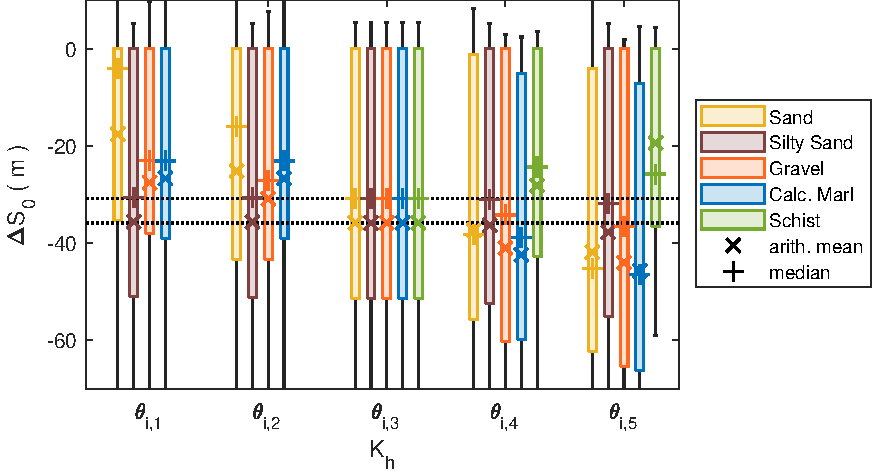
\includegraphics[width=0.8\textwidth]{./img/Fig-SensAna-K_h-DeltaS_0.pdf}
    \caption{Sensitivity of the model towards the parameter $K_h$ for all five materials $i$, measured by the error $\Delta S_0$. The corresponding parameter values $\theta_{i,j}$ are defined by Equation \eqref{Eq-ParamValCalc} and thus increase from left to right on a logarithmic scale. Each boxplot comprises the same set of piezometers. Whiskers and outliers are cut off for better perceptability. The black dotted lines mark the medians ($\bm{+}$) and arithmetic means $\bm{\times}$ of the reference parameter $\theta_{i,3}$.}
    \label{Fig-SAKhDeltaS0}

    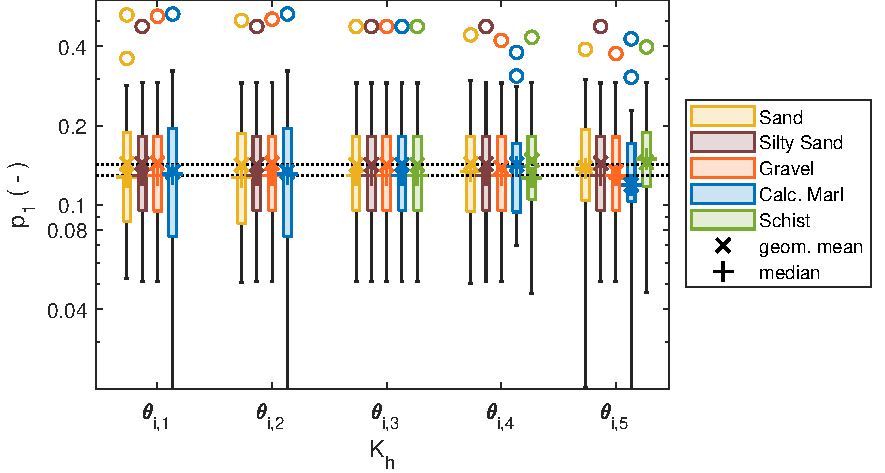
\includegraphics[width=0.8\textwidth]{./img/Fig-SensAna-K_h-p_1.pdf}
    \caption{Sensitivity of the model towards the parameter $K_h$ for all five materials $i$, measured by the error $p_1$. The corresponding parameter values $\theta_{i,j}$ are defined by Equation \eqref{Eq-ParamValCalc} and thus increase from left to right on a logarithmic scale. Each boxplot comprises the same set of piezometers. Whiskers and outliers are cut off for better perceptability. The black dotted lines mark the medians ($\bm{+}$) and arithmetic means $\bm{\times}$ of the reference parameter $\theta_{i,3}$.}
    \label{Fig-SAKhp1}
\end{figure}

\begin{figure}[p]
    \centering
    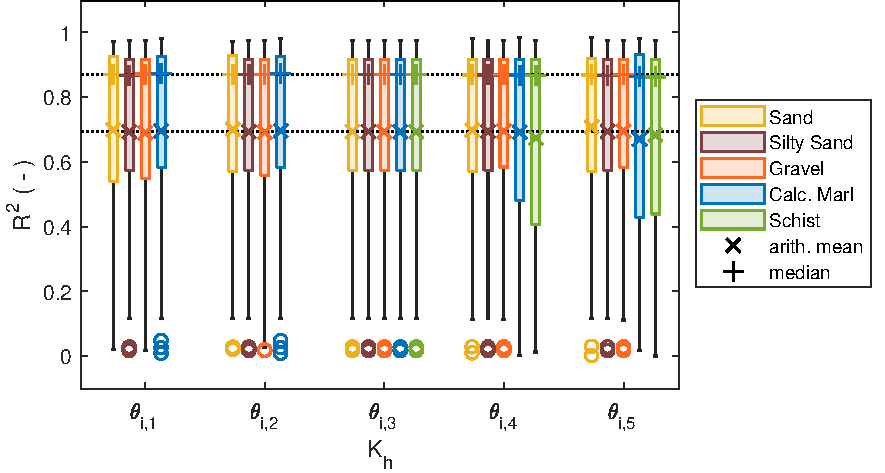
\includegraphics[width=0.8\textwidth]{./img/Fig-SensAna-K_h-R^2.pdf}
    \caption{Sensitivity of the model towards the parameter $K_h$ for all five materials $i$, measured by the error $R^2$. The corresponding parameter values $\theta_{i,j}$ are defined by Equation \eqref{Eq-ParamValCalc} and thus increase from left to right on a logarithmic scale. Each boxplot comprises the same set of piezometers. Whiskers and outliers are cut off for better perceptability. The black dotted lines mark the medians ($\bm{+}$) and arithmetic means $\bm{\times}$ of the reference parameter $\theta_{i,3}$.}
    \label{Fig-SAKhR2}
    
    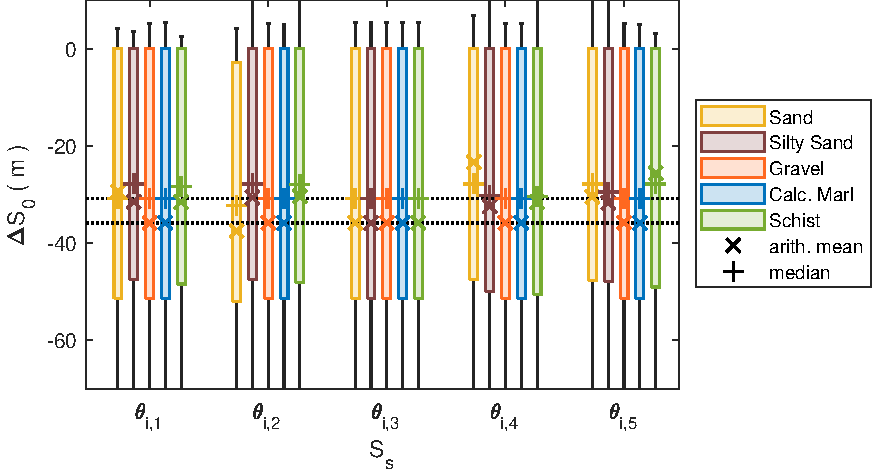
\includegraphics[width=0.8\textwidth]{./img/Fig-SensAna-S_s-DeltaS_0.pdf}
    \caption{Sensitivity of the model towards the parameter $S_s$ for all five materials $i$, measured by the error $\Delta S_0$. The corresponding parameter values $\theta_{i,j}$ are defined by Equation \eqref{Eq-ParamValCalc} and thus increase from left to right on a logarithmic scale. Each boxplot comprises the same set of piezometers. Whiskers and outliers are cut off for better perceptability. The black dotted lines mark the medians ($\bm{+}$) and arithmetic means $\bm{\times}$ of the reference parameter $\theta_{i,3}$.}
    \label{Fig-SASsDeltaS0}
\end{figure}

For the specific storage $S_s$, the model converges for all examined parameter variations in respect to the reference parameter set. 
For $\Delta S_0$ (Figure \ref{Fig-SASsDeltaS0}), all boxplots show only little variation compared to $K_h$. 
While gravel and calcareous marl seem to not have any impact on the simulation values, significant non-monotonic variations especially of the arithmetic average can be observed for the other three materials. 
The comparably large impact on the arithmetic mean can here again be explained by variations of single piezometers. 
Nonetheless, variations also occur for the respective medians, indicating shifts in the whole subset of piezometers. 
In comparison to the horizontal hydraulic conductivity (Figure \ref{Fig-SAKhp1}) the specific storage has a significantly larger impact on the slope coefficient $p_1$ (Figure \ref{Fig-SASsp1}). 
For calcareous marl and gravel only some outliers are slightly affected. For sand boxplots, means and medians show significant changes. 
For schist and silty sand these variations are even higher, for schist with an approximate factor of 5 over the full range. 
On $R^2$ (Figure \ref{Fig-SASsR2}), the specific storage also has for all materials only small impacts in average. 
For sand and schist, single piezometers however appear to be affected significantly.

\begin{figure}[p]
    \centering
    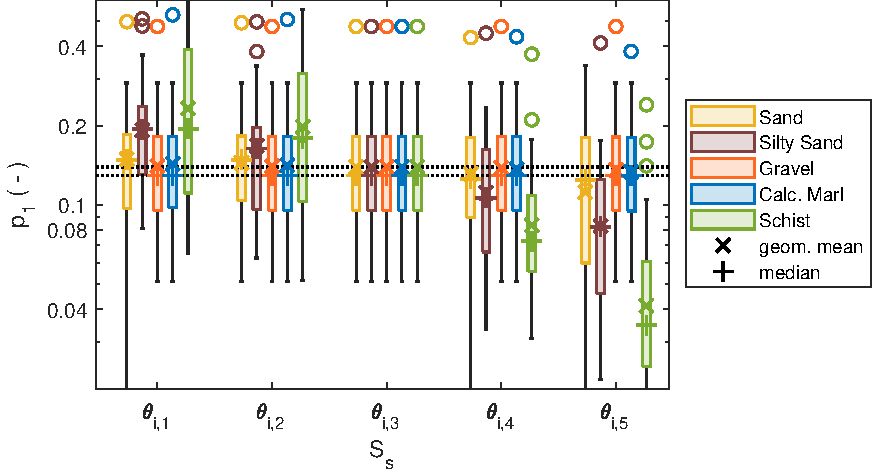
\includegraphics[width=0.8\textwidth]{./img/Fig-SensAna-S_s-p_1.pdf}
    \caption{Sensitivity of the model towards the parameter $S_s$ for all five materials $i$, measured by the error $p_1$. The corresponding parameter values $\theta_{i,j}$ are defined by Equation \eqref{Eq-ParamValCalc} and thus increase from left to right on a logarithmic scale. Each boxplot comprises the same set of piezometers. Whiskers and outliers are cut off for better perceptability. The black dotted lines mark the medians ($\bm{+}$) and arithmetic means $\bm{\times}$ of the reference parameter $\theta_{i,3}$.}
    \label{Fig-SASsp1}
    
    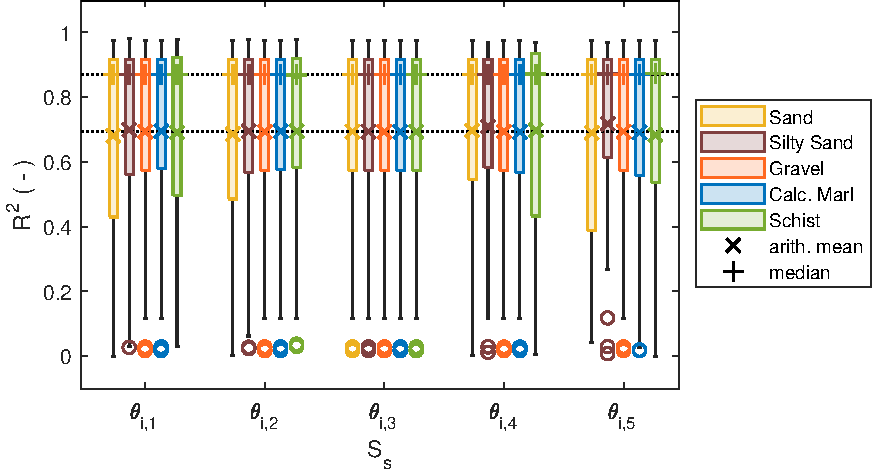
\includegraphics[width=0.8\textwidth]{./img/Fig-SensAna-S_s-R^2.pdf}
    \caption{Sensitivity of the model towards the parameter $K_h$ for all five materials $i$, measured by the error $R^2$. The corresponding parameter values $\theta_{i,j}$ are defined by Equation \eqref{Eq-ParamValCalc} and thus increase from left to right on a logarithmic scale. Each boxplot comprises the same set of piezometers. Whiskers and outliers are cut off for better perceptability. The black dotted lines mark the medians ($\bm{+}$) and arithmetic means $\bm{\times}$ of the reference parameter $\theta_{i,3}$.}
    \label{Fig-SASsR2}
\end{figure}

Finally, the scaling factor of the irrigation pumping rates $\theta_{Q,irr}$ shows on both initial offset $\Delta S_0$ (Figure \ref{Fig-SAQpDeltaS0}) and $p_1$ (Figure \ref{Fig-SAQpp1}) very large impacts. 
For $\Delta S_0$ non-monotonic behaviour can be observed, whereas for $p_1$ monotonic behaviour occurs. 
Once again, $R^2$ (Figure \ref{Fig-SAQpR2}) is affected only for single piezometers.

\begin{figure}[p]
    \centering
    \includegraphics[width=0.8\textwidth]{./img/Fig-SensAna-theta_{Q,irr}-DeltaS_0.pdf}
    \caption{Sensitivity of the model towards the parameter $\theta_{Q,irr}$, measured by the error $\Delta S_0$. The corresponding parameter values $\theta_{i,j}$ are defined by Equation \eqref{Eq-ParamValCalc} and thus increase from left to right on a logarithmic scale. Each boxplot comprises the same set of piezometers. Whiskers and outliers are cut off for better perceptability. The black dotted lines mark the medians ($\bm{+}$) and arithmetic means $\bm{\times}$ of the reference parameter $\theta_{i,3}$.}
    \label{Fig-SAQpDeltaS0}
    
    \includegraphics[width=0.8\textwidth]{./img/Fig-SensAna-theta_{Q,irr}-p_1.pdf}
    \caption{Sensitivity of the model towards the parameter $\theta_{Q,irr}$, measured by the error $p_1$. The corresponding parameter values $\theta_{i,j}$ are defined by Equation \eqref{Eq-ParamValCalc} and thus increase from left to right on a logarithmic scale. Each boxplot comprises the same set of piezometers. Whiskers and outliers are cut off for better perceptability. The black dotted lines mark the medians ($\bm{+}$) and arithmetic means $\bm{\times}$ of the reference parameter $\theta_{i,3}$.}
    \label{Fig-SAQpp1}
\end{figure}

\begin{figure}[h]
    \centering
    \includegraphics[width=0.8\textwidth]{./img/Fig-SensAna-theta_{Q,irr}-R^2.pdf}
    \caption{Sensitivity of the model towards the parameter $\theta_{Q,irr}$, measured by the error $R^2$. The corresponding parameter values $\theta_{i,j}$ are defined by Equation \eqref{Eq-ParamValCalc} and thus increase from left to right on a logarithmic scale. Each boxplot comprises the same set of piezometers. Whiskers and outliers are cut off for better perceptability. The black dotted lines mark the medians ($\bm{+}$) and arithmetic means $\bm{\times}$ of the reference parameter $\theta_{i,3}$.}
    \label{Fig-SAQpR2}
\end{figure}

All in all, the different sensitivites are summarised in Table \ref{Tab-SAOverview}. 
It can be seen, that in average $K_h$ has a significantly larger impact on $\Delta S_0$ and $S_s$ has a significantly larger impact on $p_1$. 
This goes in line with the fact that commonly $K_h$ is calibrated for the initial steady state and $S_s$ for the transient state. 
Nonetheless, smaller impacts appear also on the respective other error measure. 
This indicates that it might be reasonable to calibrate these two parameters following an alternating scheme as described in Section \ref{Sec-SubMethCal}.

Without knowledge of the effect on the single piezometer, information about the can be drawn from the here portrayed boxplots. 
Therefore, a depiction of the excessively many 27 piezometer-specific time series can here and for the further analysis be omitted. 
It can be seen that the parameters have different impacts over the modelling area. 
For the material-specific parameters this is to be expected, as the lithological units are not homogeneously distributed. 
Regarding the scaling factor for pumping rates of irrigation wells $\theta_{Q,irr}$, an analogue statement is reasonable.

For both parameter groups it can furthermore be stated that not all materials have similar impacts on the simulation results. 
In case of the hydraulic conductivity, silty sand appears to be rather negligible. 
The same applies for calcareous marl and gravel when regarding the specific storage $S_s$. 
The scaling factor $\theta_{Q,irr}$ has a significant impact on both parameters. 
For $p_1$ this is not surprising, as groundwater withdrawal in the Chtouka aquifer increases over time and an overexploitation of the aquifer is observed. 
For $\Delta S_0$ however, this is unexpected as for the initial time in 1968 only little groundwater extraction takes place. 
Therewith, the impact on the simulation results at this time should be small. 
A possible explanation for this however is that $\Delta S_0$ gives an inaccurate estimation for the targeted quantity. 
This in turn can be caused by a too inaccurate estimation of the underlying trend, also indicated by $R^2$. 
$R^2$ itself shows only little sensitivity for all parameters. 
This is reasonable, since the different parameters do not introduce new processes into the model depending on the parameter values, but rather scale the corresponding processes. 
Significant impacts on averages of $R^2$ are therewith only expectable, if the choice of parameter values is so extreme that they induce a relative binary behaviour. 
This means that for example a parameter value becomes so small that the underlying process is effectively inactivated in respect to others, or so big that it becomes extremely dominant. 
This however is a rather theoretical concept, as for a model such values probably lead to convergence errors (confer $K_h^{(Schist)}$).

Finally, basing on the previous discussions the number of parameters relevant for the model calibration can be reduced by 3: $K_h^{(Silty Sand)}$, $S_s^{(Calc. Marl)}$ and $S_s^{(Gravel)}$. 
Therewith the dimensions of the parameter space for calibration becomes 8.

\vspace{3cm}

\begin{table}[t]
    \label{Tab-SAOverview}
    \caption{Summary of the sensitivities of the different error measures $p_1$, $\Delta S_0$ and $R^2$ to the material-specific parameters $K_h$ and $S_s$ and the other parameter $\theta_{Q,irr}$. Sensitivities are measured on the following ordinal scale: $\bm{++}$: highly sensitive, $\bm{+}$: sensitive, $\bm{\circ /+}$: sensitive in only single parameters, averages and medians not significantly affected, $\bm{\circ}$: not significantly sensitive.}
    \begin{tabular}{ccccccccccccc}
        \multirow{2}{*}{Material} &  & \multicolumn{3}{c}{$K_h$}                        &  & \multicolumn{3}{c}{$S_s$}                     &                       & \multicolumn{3}{c}{$\theta_{Q,irr}$}    \\
                                  &  & $p_1$        & $\Delta S_0$    & $R^2$           &  & $p_1$        & $\Delta S_0$ & $R^2$           &                       & $p_1$     & $\Delta S_0$ & $R^2$        \\ \hline
        Calc. Marl                &  & $\bm{+}$     & $\bm{++}$       & $\bm{\circ /+}$ &  & $\bm{\circ}$ & $\bm{\circ}$ & $\bm{\circ}$    & \multicolumn{1}{c|}{} & $\bm{++}$ & $\bm{++}$    & $\bm{\circ}$ \\
        Gravel                    &  & $\bm{\circ}$ & $\bm{++}$       & $\bm{\circ}$    &  & $\bm{\circ}$ & $\bm{\circ}$ & $\bm{\circ}$    & \multicolumn{1}{c|}{} &           &              &              \\
        Sand                      &  & $\bm{+}$     & $\bm{++}$       & $\bm{\circ}$    &  & $\bm{++}$    & $\bm{+}$     & $\bm{\circ /+}$ & \multicolumn{1}{c|}{} &           &              &              \\
        Schist                    &  & $\bm{+}$     & $\bm{++}$       & $\bm{\circ /+}$ &  & $\bm{++}$    & $\bm{+}$     & $\bm{\circ /+}$ & \multicolumn{1}{c|}{} &           &              &              \\
        Silty Sand                &  & $\bm{\circ}$ & $\bm{\circ /+}$ & $\bm{\circ}$    &  & $\bm{++}$    & $\bm{+}$     & $\bm{\circ /+}$ & \multicolumn{1}{c|}{} &           &              &             
    \end{tabular}
\end{table}

%%%%%%%%%%%%%%%%%%%%%%%%%%%%%%%%%%%%%%%%%%%%%%%%%%%%%%%%%%%%%%%%%%

\section{Calibration}

The calibration is conducted according to Section \ref{Sec-SubMethCal}. 
In total, 310 simulations are conducted over 7 iteration steps. 
Figure \ref{Fig-CalibResults} shows the results during the calibration process, displayed through the respective arithmetic ($\Delta S_0$) and geometric ($p_1$) averages. 
For comparison, the arithmetic mean of the $RMSE$ is plotted as well (Section \ref{Sec-DisEM}). 
Of the in total 7 iteration steps the last one yields results that are varying only slightly. 
Depicted are the simulation results of the respectively picked parameter sets. 
The first six iteration steps are shown aggregated, while the last is shown in its entirety. 
The partly large variations (especially at the end of iteration 5) stem from adjustments to the parameter ranges. 
This also causes the large jump between $K_h^{(Calc. Marl)}$ and $K_h^{(Sand)}$. 
In the end of the calibration, four different values of $\theta_{Q,irr}$ are compared: factors of 1.0, 1.3, 1.5 and 1.7. 
As can be seen, this parameter highly impacts the final result. 
As final parameter set, $\theta_{Q,irr}=1.3$ is taken, since it represents the supposedly most reasonable trade-off between acknowledged uncertainty of $\dot{M}_{irr}$ and a good result of the calibrated model. 
This is important, as for the real application time proceeds. 
Therewith, measuring and estimation techniques of the pumping rates are further developed and thus vary, leading to a time-dependence of this factor. 
For the other calibrated parameters this issue however does not arise, since these represent material properties of the lithological units and can therefore be assumed as constant over time. 
The final parameter set is listed in Table \ref{Tab-FinalParams}.

\begin{figure}[h]
    \centering
    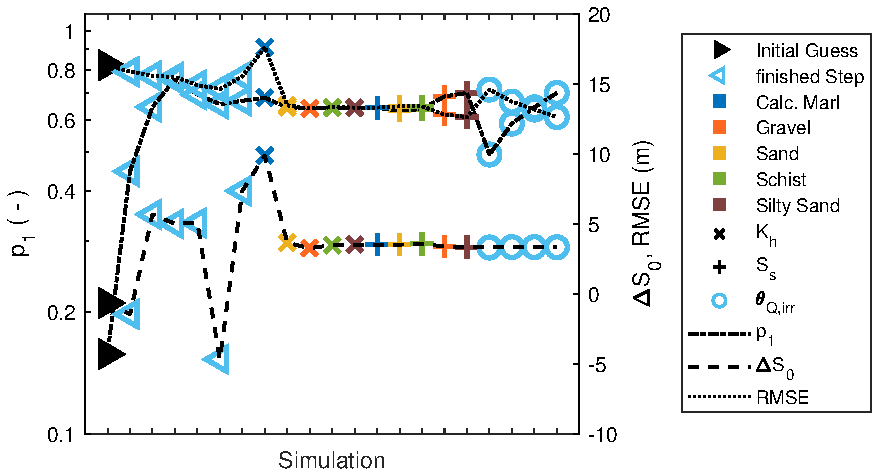
\includegraphics[width=0.8\textwidth]{./img/Fig-CalibResults.pdf}
    \caption{The results of the calibration process for the error measures $p_1$ and $\Delta S_0$. The $RMSE$ is plotted for comparison. Along the $x$-axis advances the calibration process, starting on the left with the initial simulation results. All seven executed iterations are depicted. Of these, the first six are shown aggregated as final iteration result. For the last iteration, for each of the material parameters the best-fitting result is shown. The last four instances mark final variations of $\theta_{Q,irr}$.}
    \label{Fig-CalibResults}
\end{figure}

\begin{table}[h]
    \label{Tab-FinalParams}
    \caption{The values of final parameter set.}
    \begin{tabular}{cccc}
    Material   & $K_h \; \textrm{( m )}$ & $S_s \; \textrm{m}^{-1}$    & $\theta_{Q,irr} \; \textrm{( - )}$ \\ \hline
    Sand       & 0.00003                 & \multicolumn{1}{c|}{0.002}  & 1.3                                \\
    Silty Sand & 0.000009                & \multicolumn{1}{c|}{0.0002} &                                    \\
    Gravel     & 0.005                   & \multicolumn{1}{c|}{0.003}  &                                    \\
    Calc. Marl & 0.0004                  & \multicolumn{1}{c|}{0.0005} &                                    \\
    Schist     & 0.000006                & \multicolumn{1}{c|}{0.0003} &                                   
    \end{tabular}
    \end{table}

%%%%%%%%%%%%%%%%%%%%%%%%%%%%%%%%%%%%%%%%%%%%%%%%%%%%%%%%%%%%%%%%%%

\section{Discussion of Error Measures}
\label{Sec-DisEM}

In Figure \ref{Fig-CalibResults} the $RMSE$ is also displayed for comparison. 
Along with the calibration decisions, the $RMSE$ shows from the first iteration on a monotonic decline in value. 
Only for the final variation of $\theta_{Q,irr}$ an partwise increase can be observed. 
This one however is analogue to the behaviour of $p_1$. 
Obviously, the $RMSE$ seems to lead to analogue calibration decisions. 
However it may here be noted, that in the regarded graph only one out of five to seven options is depicted. 
Therefore, it is not possible to determine, if a better fit could have been found along the way. 
Nonetheless, based on this perception, the $RMSE$ seems equally fit for calibration as $\Delta S_0$ and $p_1$ - or vise versa. 
However, the here examined calibrating process belongs to a particular model with seemingly only little interactions between the different parameters. 
For other usecases, especially when parameters significantly impact two of the error measures at a time, they might unfold a higher potential.

Furthermore it can be stated that the initial implementation of the error measures is more laborious. 
For the experienced programmer however, this may not be a significant impact. 
Also, the more complex computations require more resources. 
For most applications, the computational costs of the simulations might still be significantly higher.

The underlying assumption of this method is that simulation values $S$ and observations $E$ show a large enough correlation. 
This should be a reasonable assumption, as a model is designed to correlate to observations. 
Additionally, with $R^2$ a factor for the assessment of this assumption in a particular case is given.

%%%%%%%%%%%%%%%%%%%%%%%%%%%%%%%%%%%%%%%%%%%%%%%%%%%%%%%%%%%%%%%%%%

\section{Discussion Lumping of Irrigation Wells}
\label{Sec-DisLIW}

In the current model a total of 5498 wells are included, each as a single point with a corresponding time series. 
As this amount of data was assumed to cost an extensive portion of computational resources, the possibility of lumping of the groundwater wells should be examined. 
As the spatial extents of the areas in which groundwater pumping occurs vary over time, this would require several layers of different shapefiles as for the irrigation zones. 
The loading of the original 5498 pointwise timeseries however proves to take approximately 5 minutes, everytime that changes are made to the underlying data. 
In case of a lumped representation, each layer would have to be imported seperately by hand. 
This procedure however takes more than the automatic point-wise reading. 
Therefore the approach is deemed unfavourable and is thus not further examined in this study.